\documentclass[12pt]{article}

\usepackage{amsmath, amssymb, amsthm, enumerate, graphicx}
\usepackage[usenames,dvipsnames]{color}
\usepackage{bm}
\usepackage[colorlinks=true,urlcolor=blue]{hyperref}
\usepackage{geometry}
\geometry{margin=1in}
\usepackage{float}
\usepackage{graphics}
\setlength{\marginparwidth}{2.15cm}
\usepackage{booktabs}
\usepackage{enumitem}
\usepackage{epsfig}
\usepackage{setspace}
\usepackage{parskip}
\usepackage[normalem]{ulem}
\usepackage{tikz}
\usetikzlibrary{positioning, arrows, automata}
\usepackage{pgfplots}
\usepackage[font=scriptsize]{subcaption}
\usepackage{float}
\usepackage[]{algorithm2e}
\usepackage{environ}
\usepackage{bbm}
\usepackage{graphicx}
\usepackage{titling}
\usepackage{url}
\usepackage{xcolor}
\usepackage{lipsum}
\usepackage{lastpage}
\usepackage[colorlinks=true,urlcolor=blue]{hyperref}
\usepackage{multicol}
\usepackage{tabularx}
\usepackage{comment}
\usepackage[utf8]{inputenc}
\usepackage{amssymb}
\usepackage{setspace}
\usepackage{marvosym}
\usepackage{wrapfig}
\usepackage{datetime}
\usepackage[many]{tcolorbox}
\usepackage{array}
\usepackage{multirow}
\usepackage{wasysym}
\usepackage{cancel}

\usepackage{listings}
\usepackage{color}
\usepackage[thinlines]{easytable}
\usepackage{lastpage}

\newcommand{\R}{\mathbb{R}}
\newcommand{\blackcircle}{\tikz\draw[black,fill=black] (0,0) circle (1ex);}
\renewcommand{\circle}{\tikz\draw[black] (0,0) circle (1ex);}


\usetikzlibrary{positioning,calc}


%-------------------------------------------------------------------------------
% Custom commands
\usepackage{xcolor} %hilight
\newcommand{\hilight}[1]{\colorbox{yellow}{#1}}
%-------------------------------------------------------------------------------

%%BEGINSOLUTION
% To delete solutions from the TeX file, do:
% sed '/\%\%BEGINSOLUTION/,/\%\%ENDSOLUTION/d' main.tex > out.tex
%%ENDSOLUTION
\newtcolorbox[]{solution}[1][]{%
    breakable,
    enhanced,
    colback=white,
    title=Solution,
    #1
}
\begin{document}
\section*{}
\begin{center}
  \centerline{\textsc{\LARGE  Homework 3 Template}}
\end{center}

Use this template to record your answers for Homework 3.  Add your answers using \LaTeX and then save your document as a PDF to upload to Gradescope.  You are required to use this template to submit your answers.  \textbf{You should not alter this template in any way} other than to insert your solutions.  You must submit all \pageref{LastPage} pages of this template to Gradescope.  Do not remove the instructions page(s).  Altering this template or including your solutions outside of the provided boxes can result in your assignment being graded incorrectly.

You should also export your code as a .py file and upload it to the \textbf{separate} Gradescope coding assignment. Remember to mark all teammates on \textbf{both} assignment uploads through Gradescope.

\section*{Instructions for Specific Problem Types}

On this homework, you must fill in blanks for each problem. Please make sure your final answer is fully included in the given space.  \textbf{Do not change the size of the box provided.}  For short answer questions you should \textbf{not} include your work in your solution.  Only provide an explanation or proof if specifically asked.

\begin{quote}
\textbf{Fill in the blank:} What is the course number?

\begin{tcolorbox}[fit,height=1cm, width=4cm, blank, borderline={1pt}{-2pt},nobeforeafter]
    \begin{center}\huge10-703\end{center}
    \end{tcolorbox}
\end{quote}

\newpage

\section*{Problem 0: Collaborators}
Enter your team members' names and Andrew IDs in the boxes below. If you worked in a team with fewer than three people, leave the extra boxes blank.

Name 1: \begin{tcolorbox}[fit,height=1cm, width=5cm, blank, borderline={1pt}{1pt},nobeforeafter]
    \begin{center}
    \vspace{3mm}
    \large{Leandro Lopez Leon}
    \end{center}
\end{tcolorbox}
Andrew ID 1: \begin{tcolorbox}[fit,height=1cm, width=5cm, blank, borderline={1pt}{1pt},nobeforeafter]
    \begin{center}
    \vspace{3mm}
    \large{lslopez}
    \end{center}
\end{tcolorbox}
\vspace{0.5cm}
\vspace{0.5cm}
%\begin{solution}
%\centering
%\begin{tabular}{c|c|c}
%     & name & Andrew ID \\
%     \hline
%    You                 & \hspace{10em}  &   %\hspace{6em}@andrew.cmu.edu \\
%    Collaborator 1 (optional) & \hspace{10em} & %\hspace{6em}@andrew.cmu.edu\\
%    Collaborator 2 (optional) & \hspace{10em} & %\hspace{6em}@andrew.cmu.edu\\
%\end{tabular}
%\end{solution}
\newpage
\section*{Problem 1: CMA-ES (45 pt)}
\subsection*{1.1 Plot of CMA-ES on simple objective function (20 pt)}
\begin{tcolorbox}[fit,height=30em, width=40em, blank, borderline={1pt}{1pt},nobeforeafter]
            \begin{center}
            \vspace*{0.4cm}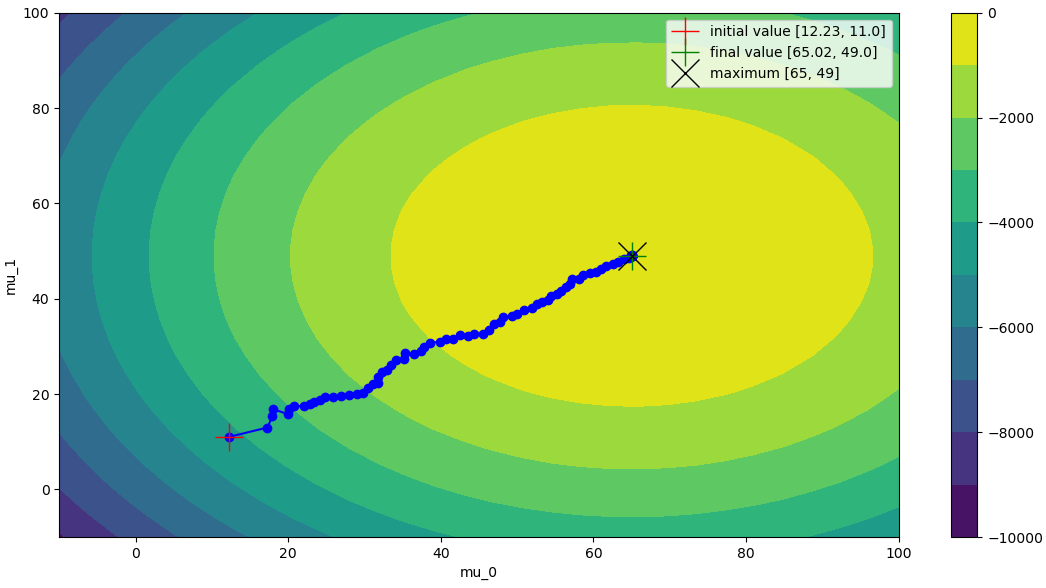
\includegraphics[height= 12cm, width=15.5cm]{q1-1}
            \end{center}
            \end{tcolorbox}
            
\subsection*{1.2 RL reward of fixed policies (10 pt)}

$x = (-1, -1, -1, -1, -1)$ : \begin{tcolorbox}[fit,height=1cm, width=5cm, blank, borderline={1pt}{1pt},nobeforeafter]
    \begin{center}
    \vspace{3mm}
    \large{15.6}
    \end{center}
\end{tcolorbox} \\
$x = (1, 0, 1, 0, 1)$ : \hspace{3.5em} \begin{tcolorbox}[fit,height=1cm, width=5cm, blank, borderline={1pt}{1pt},nobeforeafter]
    \begin{center}
    \vspace{3mm}
    \large{14.4}
    \end{center}
\end{tcolorbox} \\
$x = (0, 1, 2, 3, 4)$ : \hspace{3.5em} \begin{tcolorbox}[fit,height=1cm, width=5cm, blank, borderline={1pt}{1pt},nobeforeafter]
    \begin{center}
    \vspace{3mm}
    \large{9.4}
    \end{center}
\end{tcolorbox}

\subsection*{1.3 Plot of CMA-ES on Cartpole (15 pt)}
\begin{tcolorbox}[fit,height=30em, width=40em, blank, borderline={1pt}{1pt},nobeforeafter]
    \begin{center}
    \vspace*{0.4cm}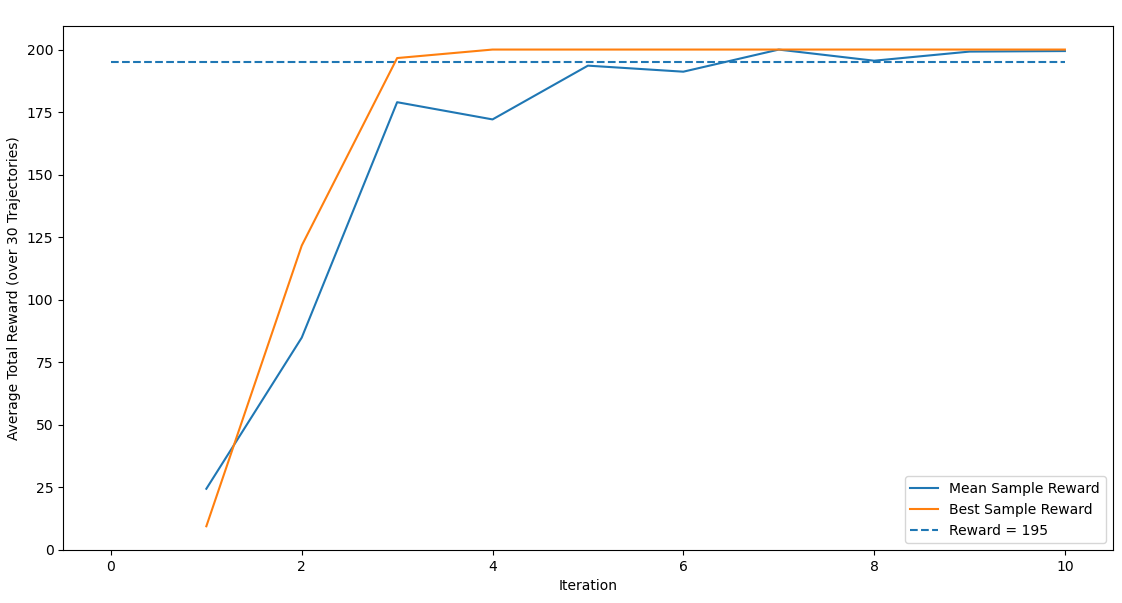
\includegraphics[height= 12cm, width=15.5cm]{q1-3}
    \end{center}
    \end{tcolorbox}
    
\newpage
\section*{Problem 2: Behavior Cloning and DAGGER (36 pt)}
\subsection*{2.1 Behavior Cloning (16 pt)}

\subsection*{2.1.1 Plot Behavior Cloning (8 pt)}
\begin{tcolorbox}[fit,height=20em, width=40em, blank, borderline={1pt}{1pt},nobeforeafter]
            \begin{center}
            %YOUR SOLUTION HERE% 
            \end{center}
            \end{tcolorbox}
            
\subsection*{2.1.2 Plot Behavior Cloning with Varying Expert Episodes (8 pt)}

\begin{tcolorbox}[fit,height=24em, width=40em, blank, borderline={1pt}{1pt},nobeforeafter]
            \begin{center}
            %YOUR SOLUTION HERE% 

\end{center}
\end{tcolorbox}


\subsection*{2.2 DAGGER (20 pt)}
\subsection*{2.2.1 Plot DAGGER (8 pt)}
\begin{tcolorbox}[fit,height=20em, width=40em, blank, borderline={1pt}{1pt},nobeforeafter]
            \begin{center}
            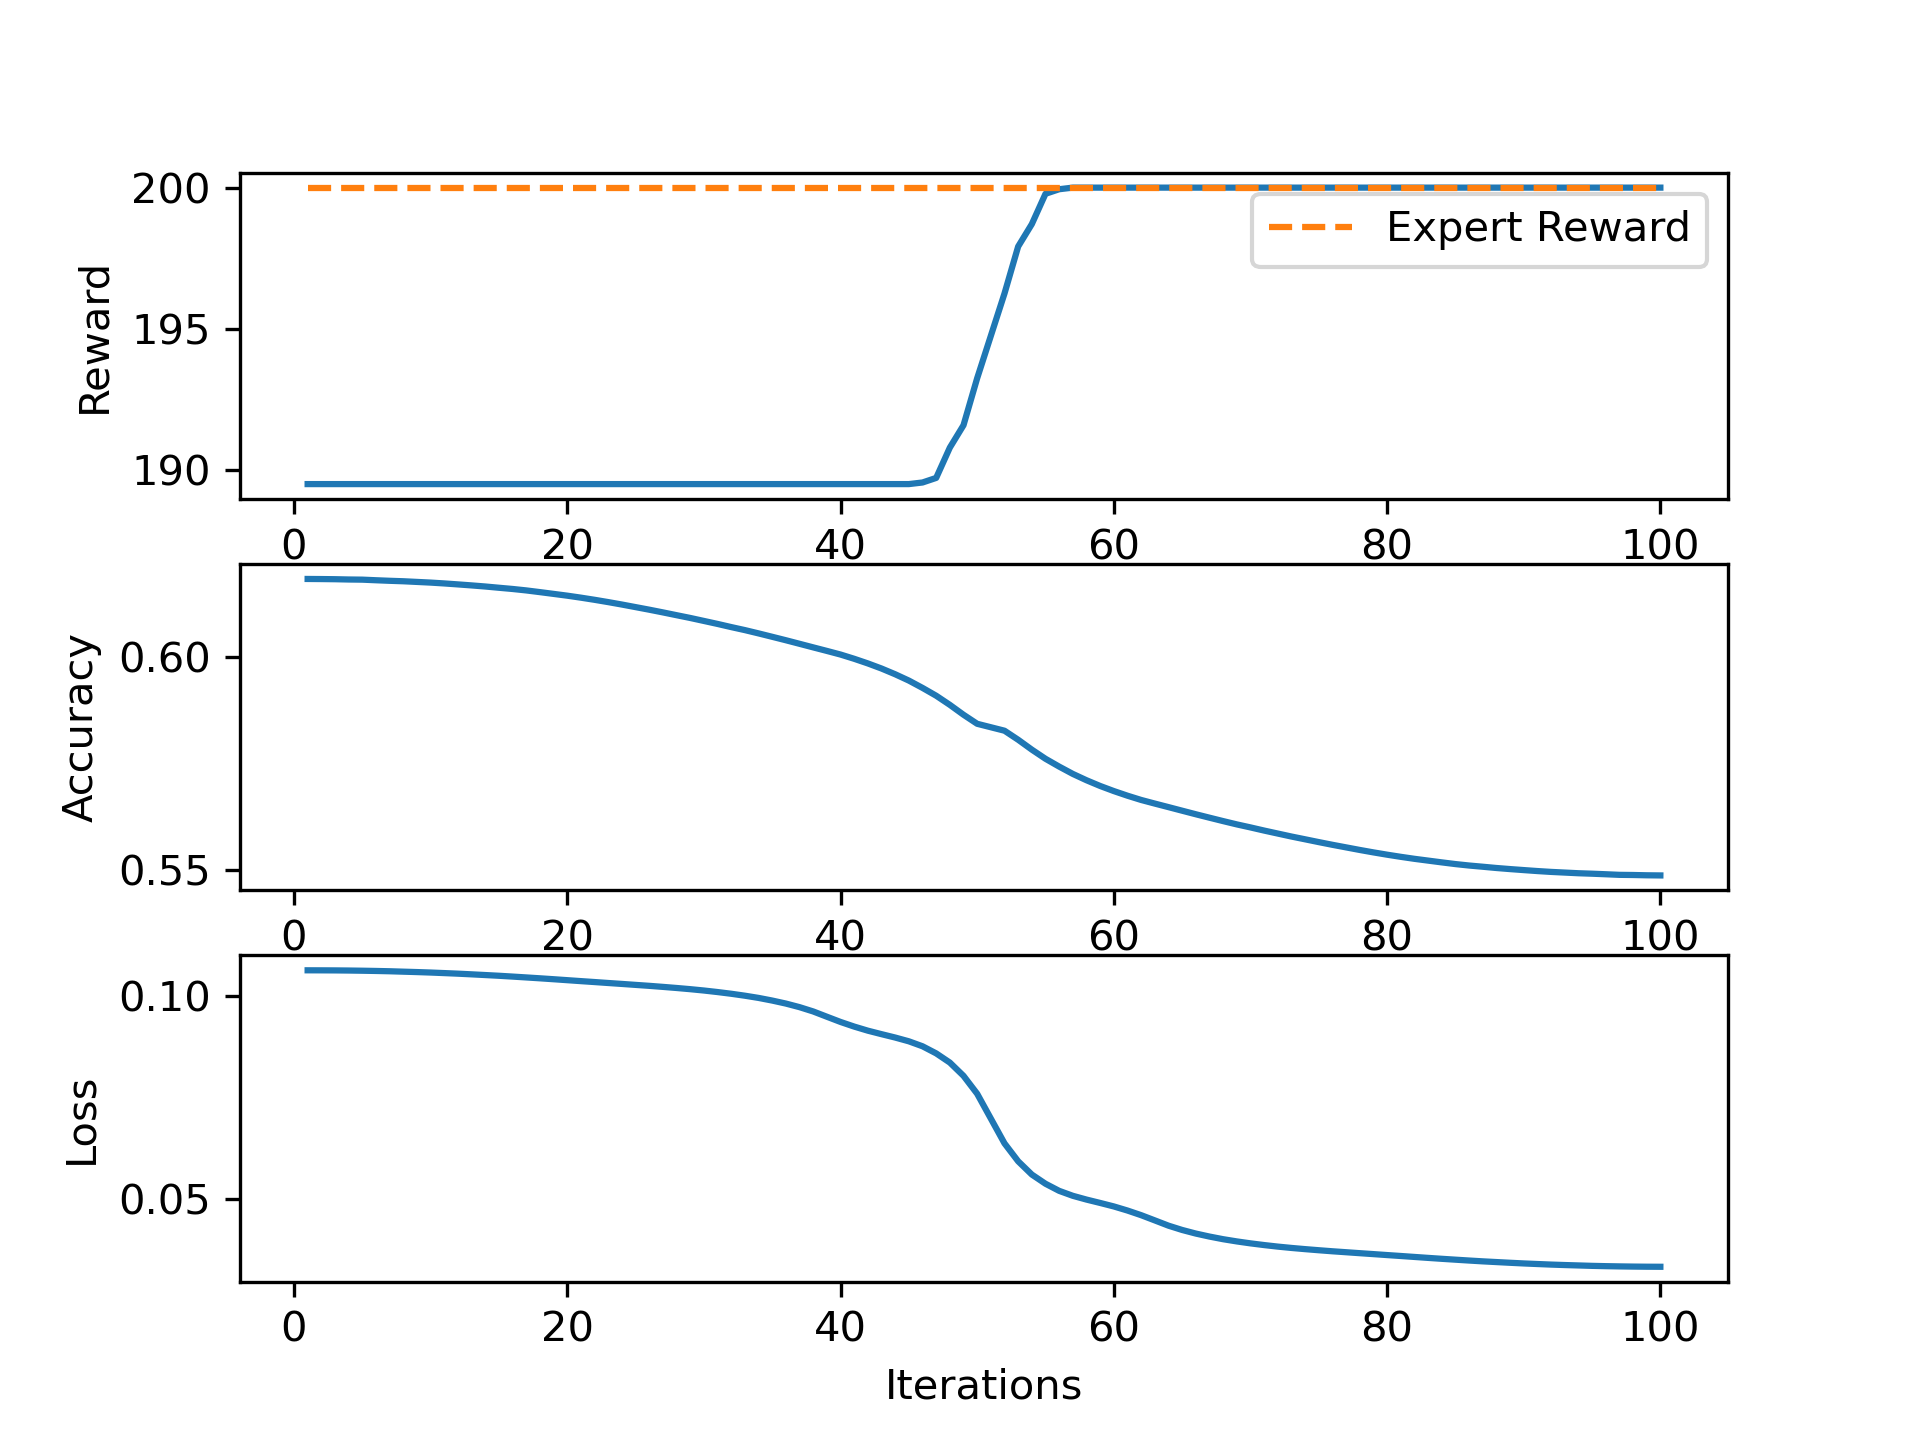
\includegraphics[height= 12cm, width=15.5cm]{q2-2-1}
            \end{center}
            \end{tcolorbox}
            
\subsection*{2.2.2 Plot DAGGER with Varying Expert Episodes (8 pt)}
\begin{tcolorbox}[fit,height=25em, width=40em, blank, borderline={1pt}{1pt},nobeforeafter]
            \begin{center}
            %YOUR SOLUTION HERE%
\end{center}
\end{tcolorbox}

\subsection*{2.2.3 Compare Behavior Cloning and DAGGER (4 pt)}
\begin{tcolorbox}[fit,height=24em, width=40em, blank, borderline={1pt}{1pt},nobeforeafter]
            \begin{center}
            % YOUR SOLUTION HERE%

\end{center}
\end{tcolorbox}

\clearpage
\section*{Problem 3: Goal-Conditioned BC (45 pt)}

\subsection*{3.1 Build Goal-Conditioned Task (3 pt)}
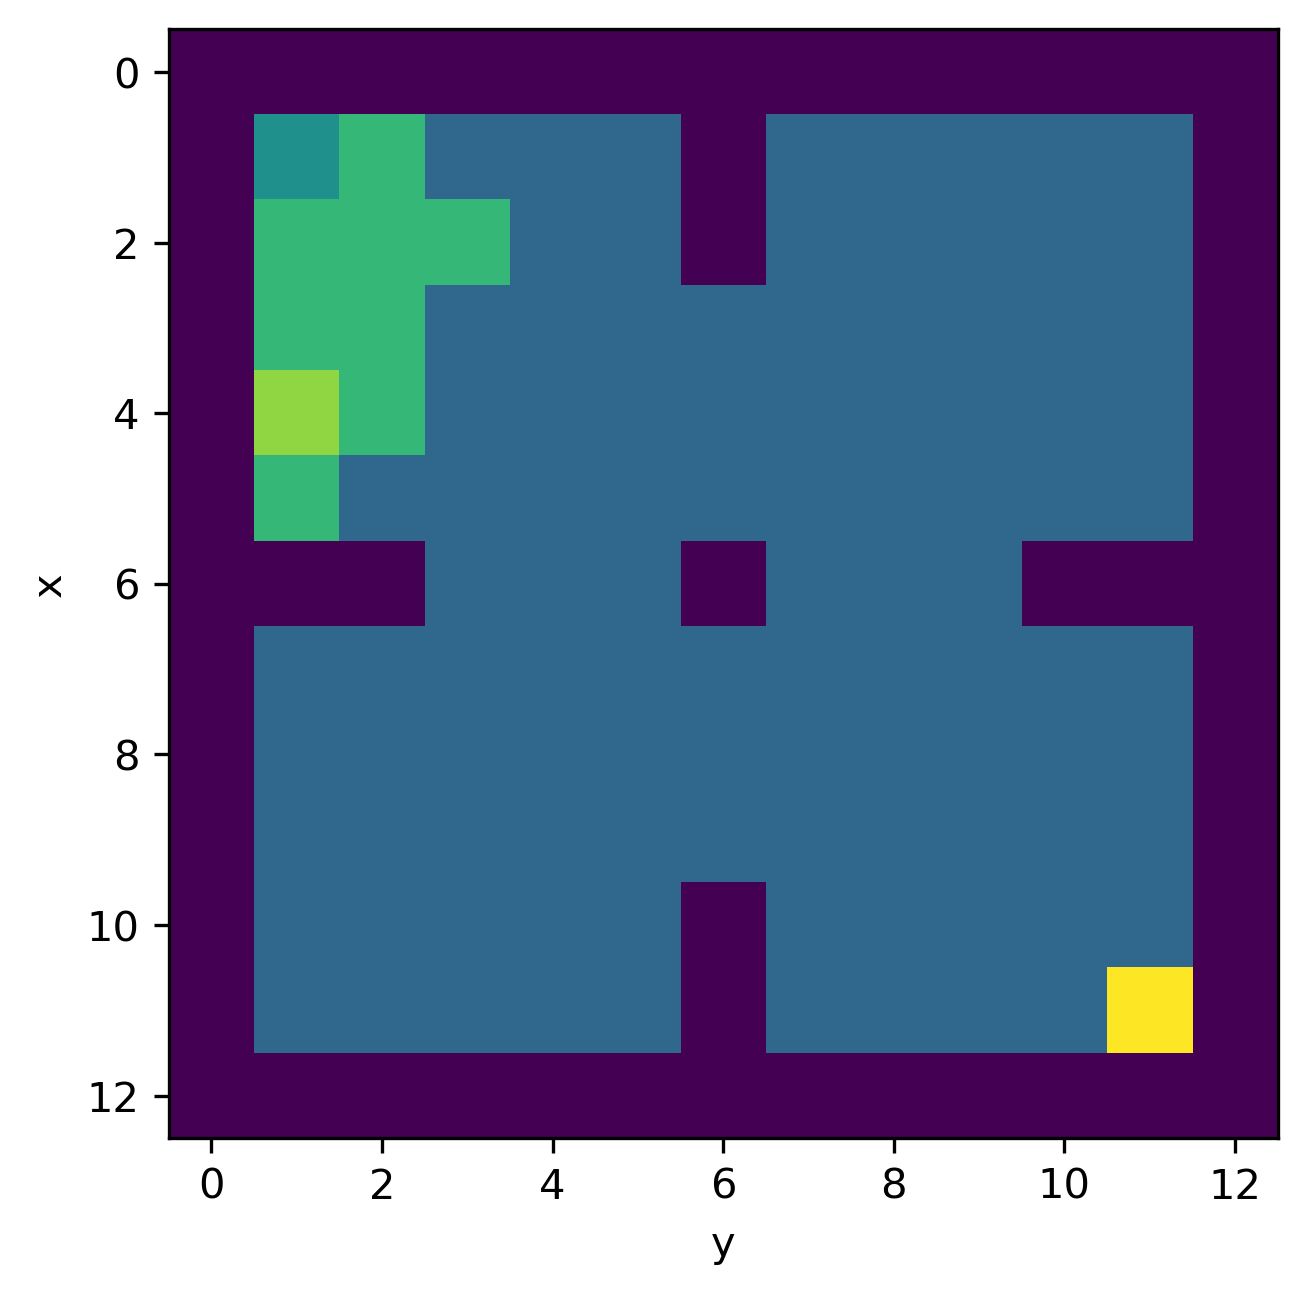
\includegraphics[height= 15.5cm, width=15.5cm]{p3-1-1}



\subsection*{3.2 Run Search Algorithm as Expert (8 pt)}

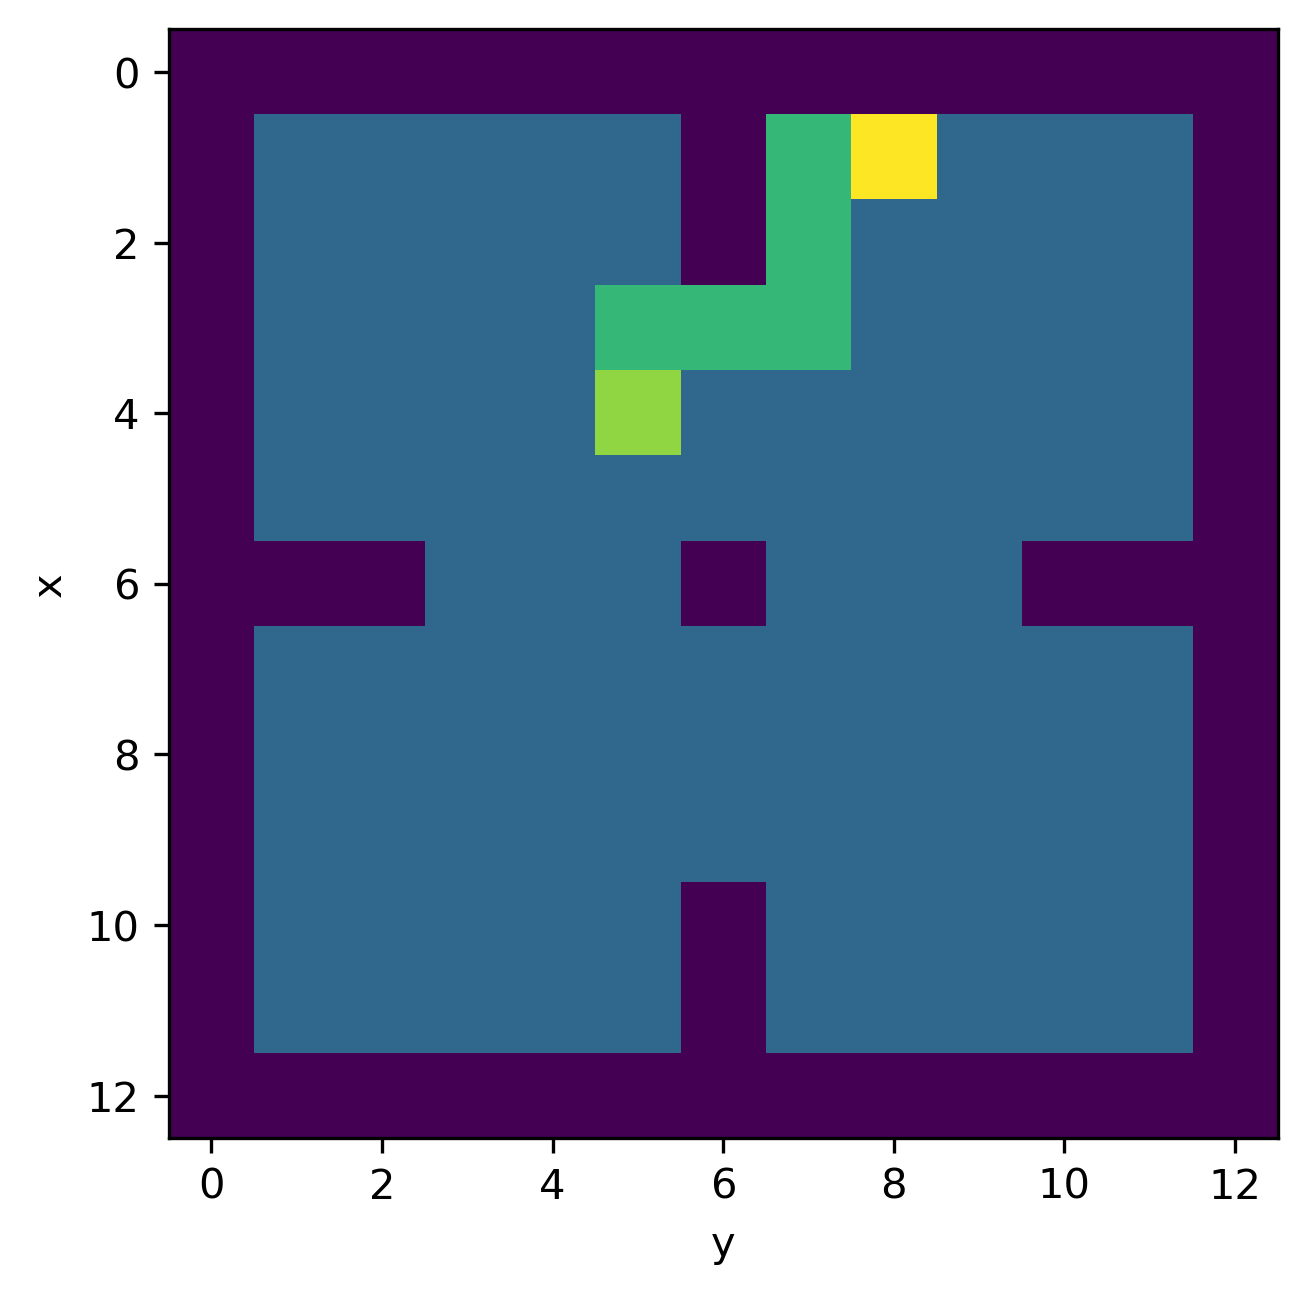
\includegraphics[height= 5cm, width=5cm]{p3-2-0}
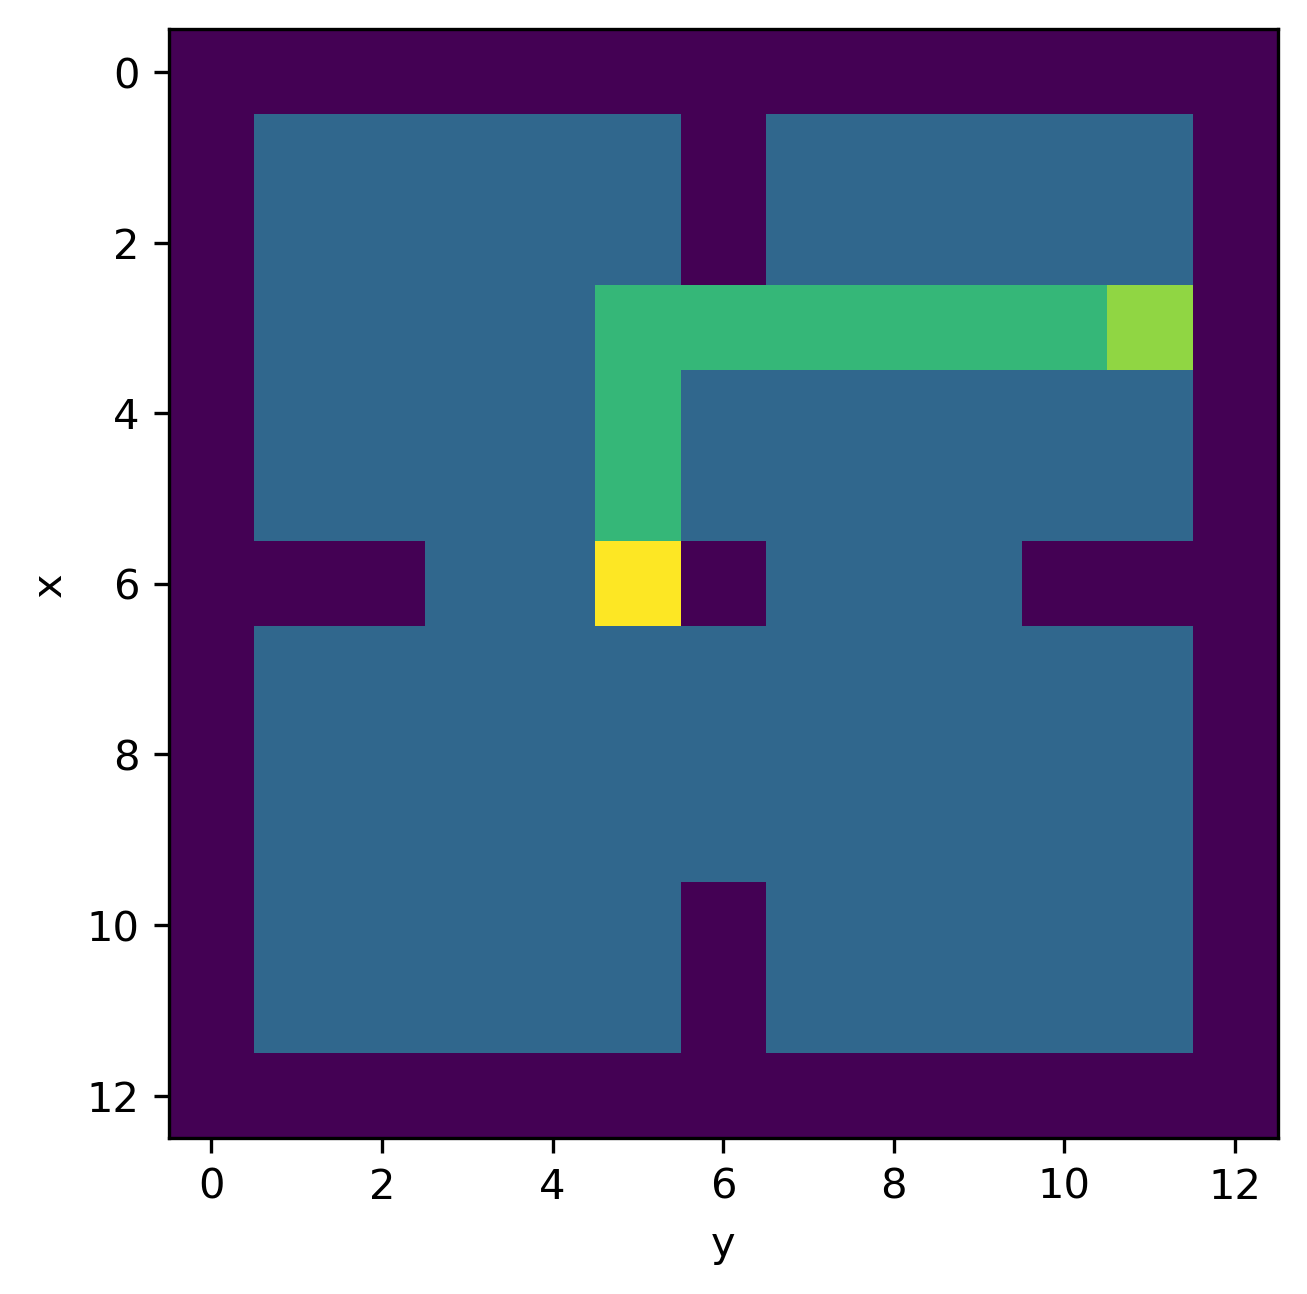
\includegraphics[height= 5cm, width=5cm]{p3-2-1}
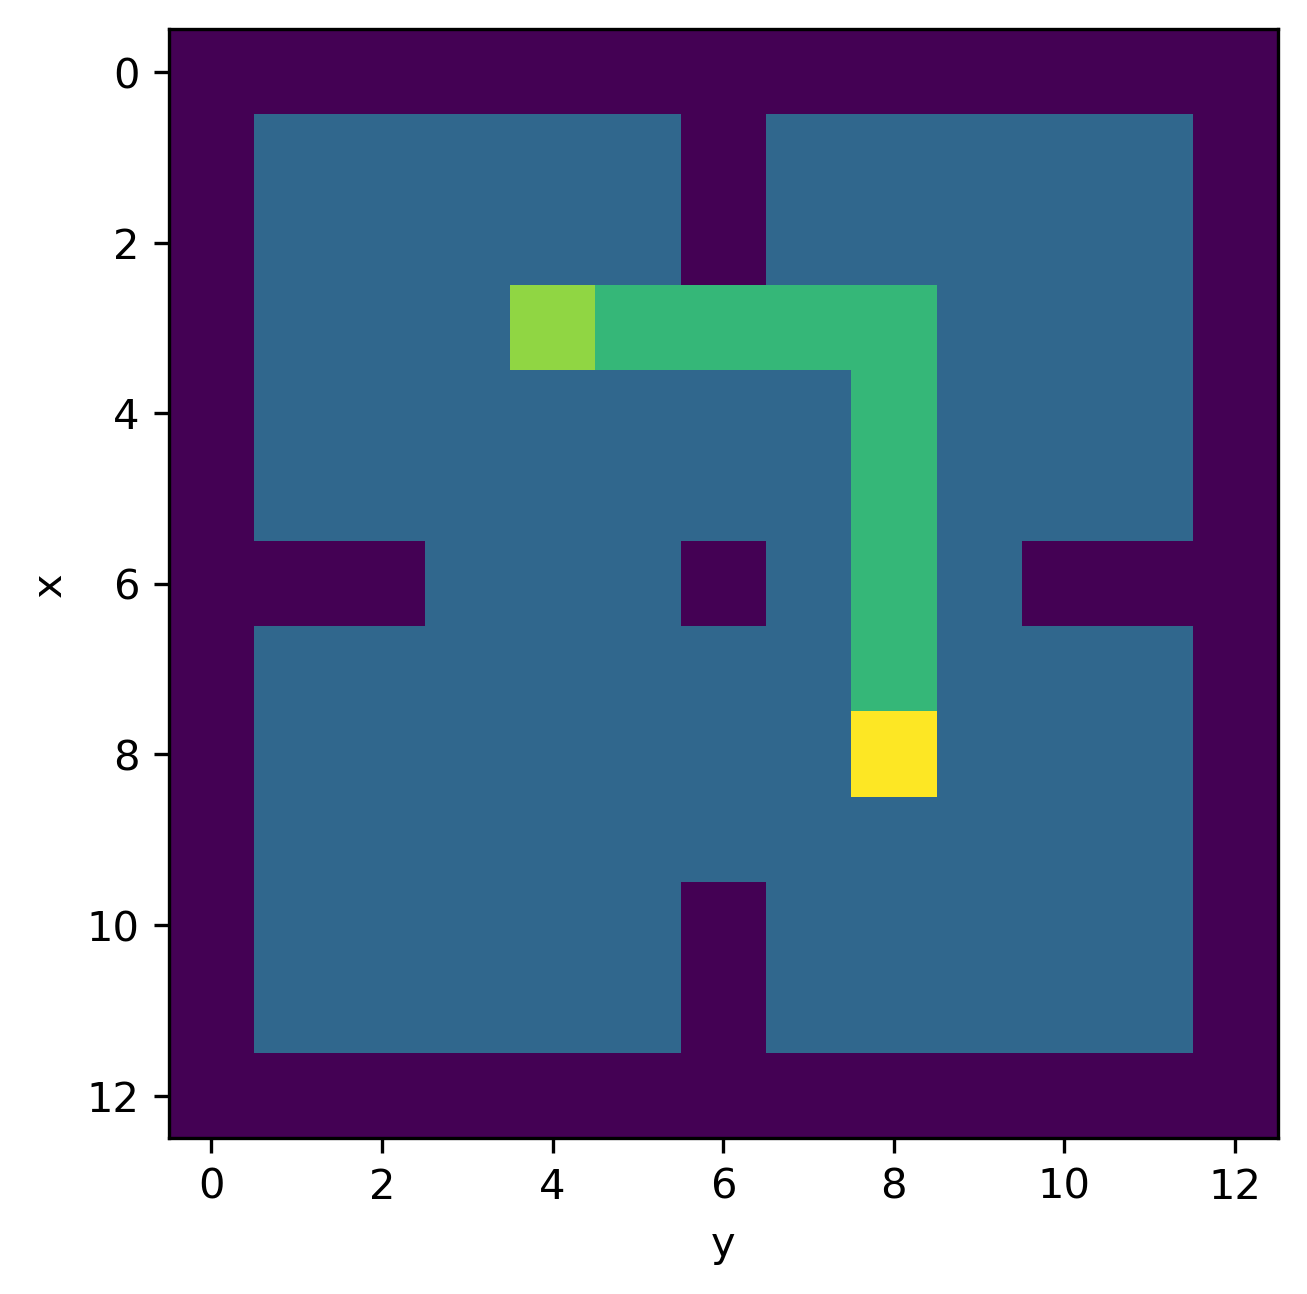
\includegraphics[height= 5cm, width=5cm]{p3-2-2} 
\\
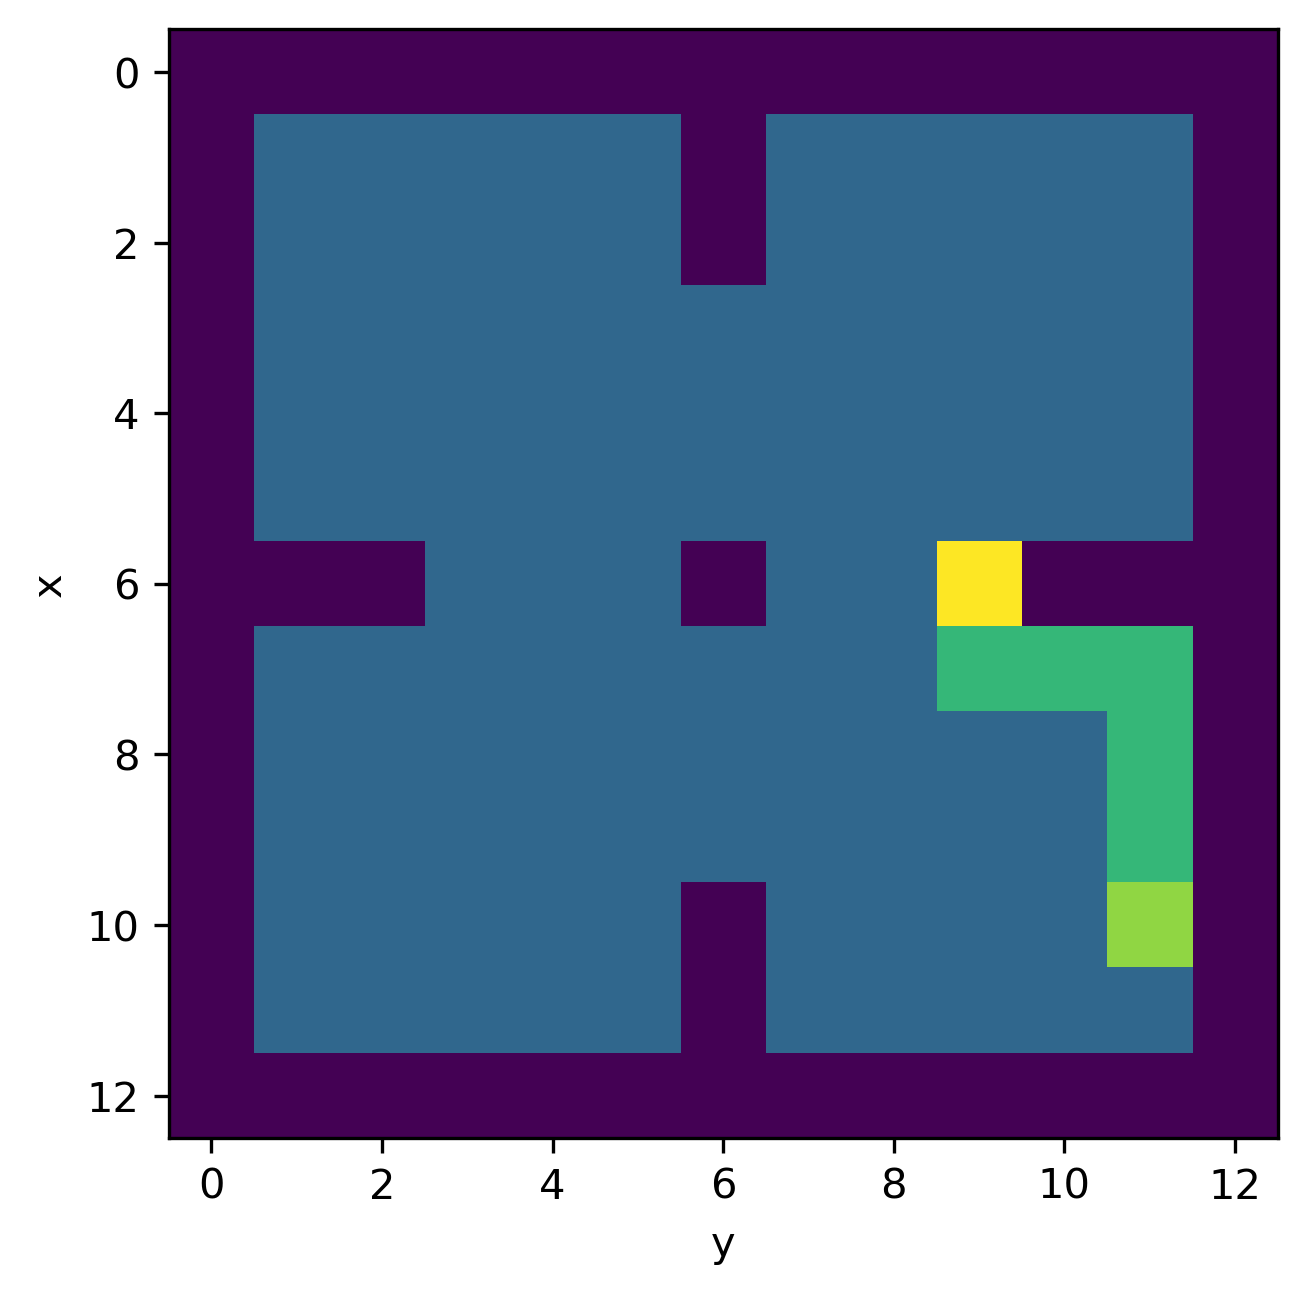
\includegraphics[height= 5cm, width=5cm]{p3-2-3}
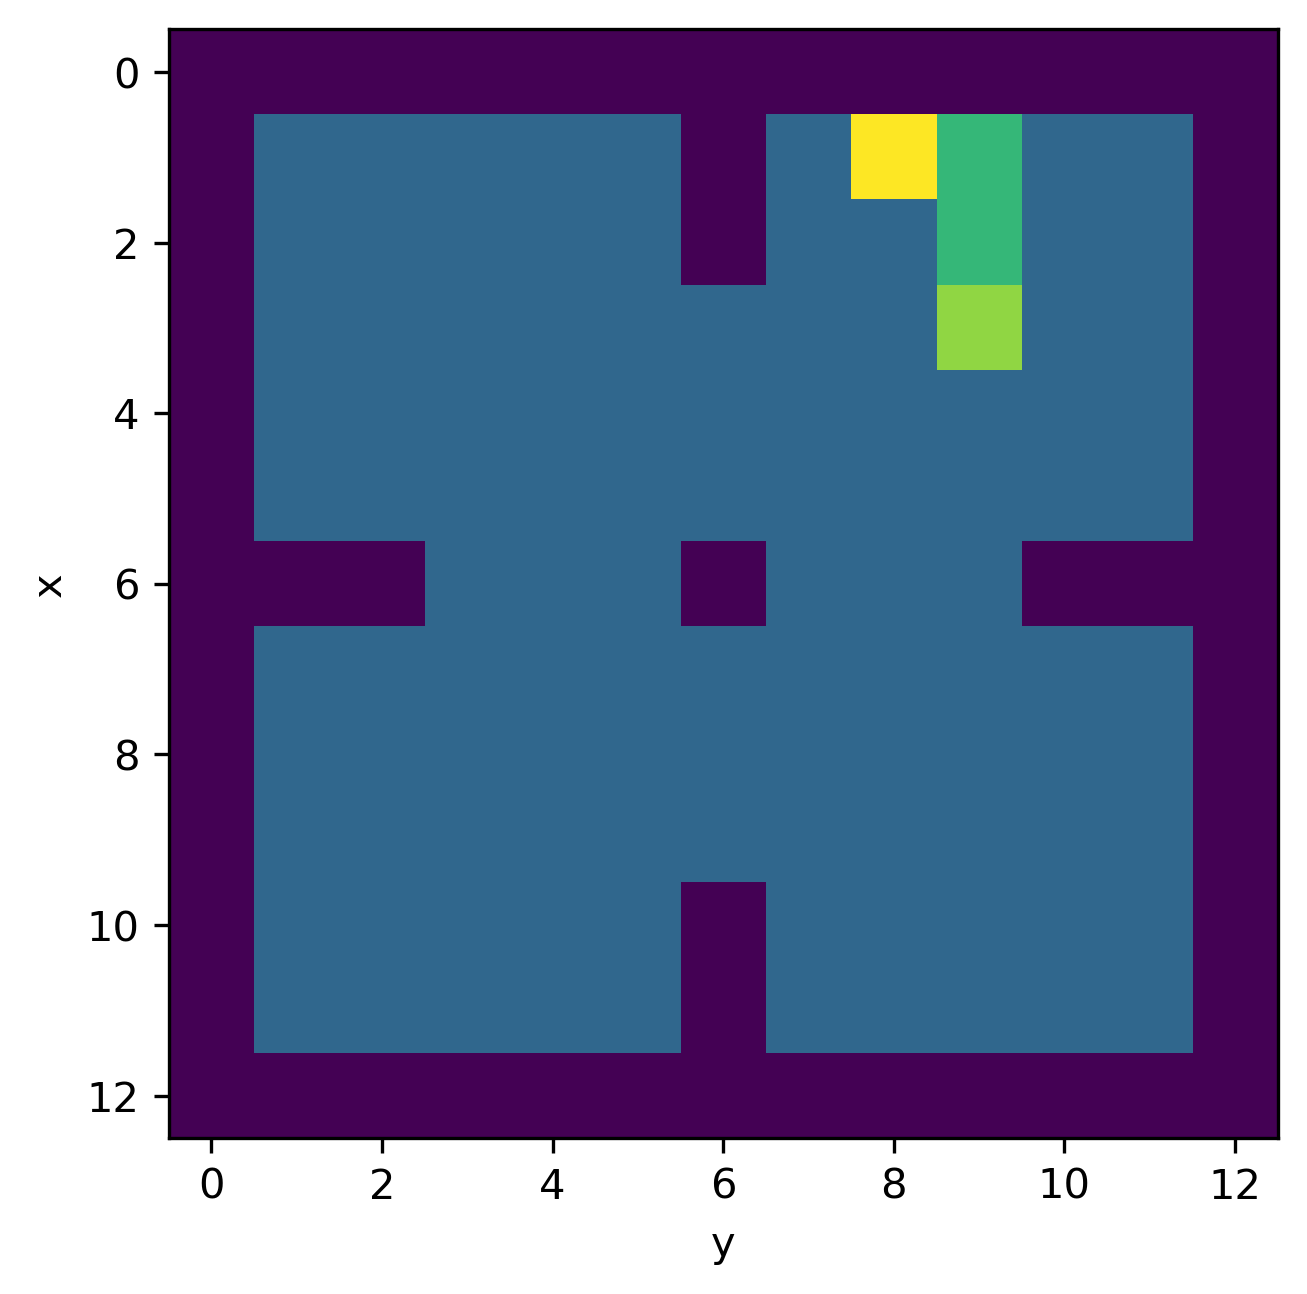
\includegraphics[height= 5cm, width=5cm]{p3-2-4}
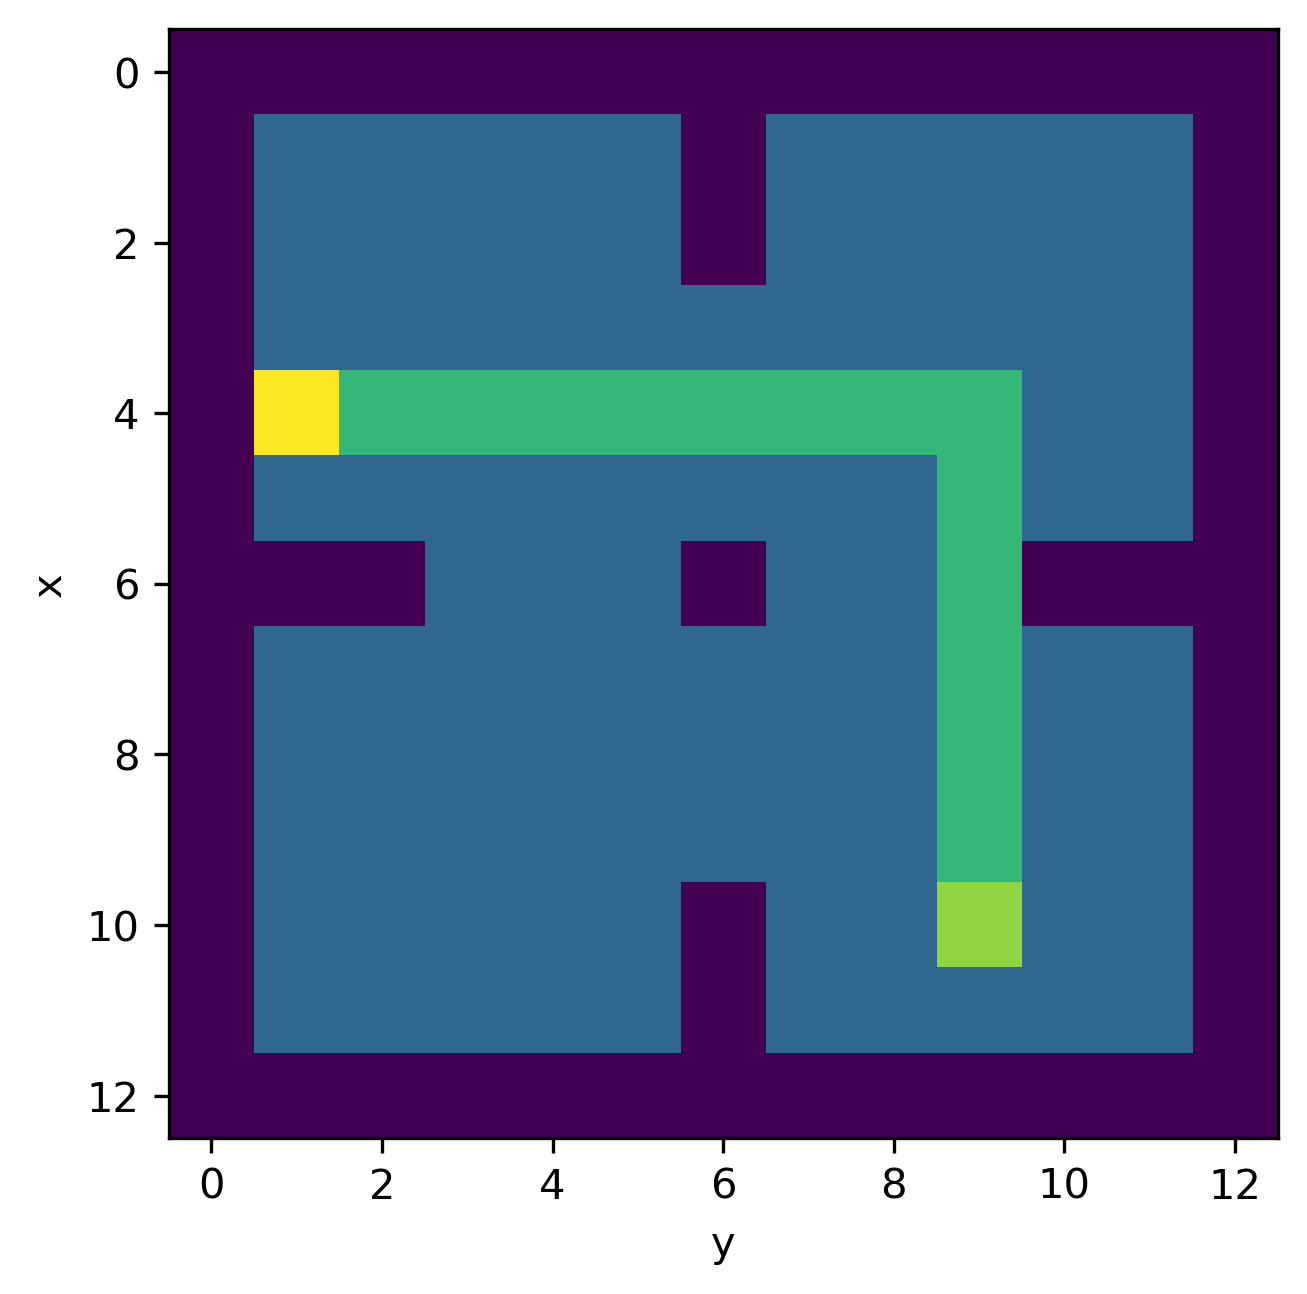
\includegraphics[height= 5cm, width=5cm]{p3-2-5}
\\

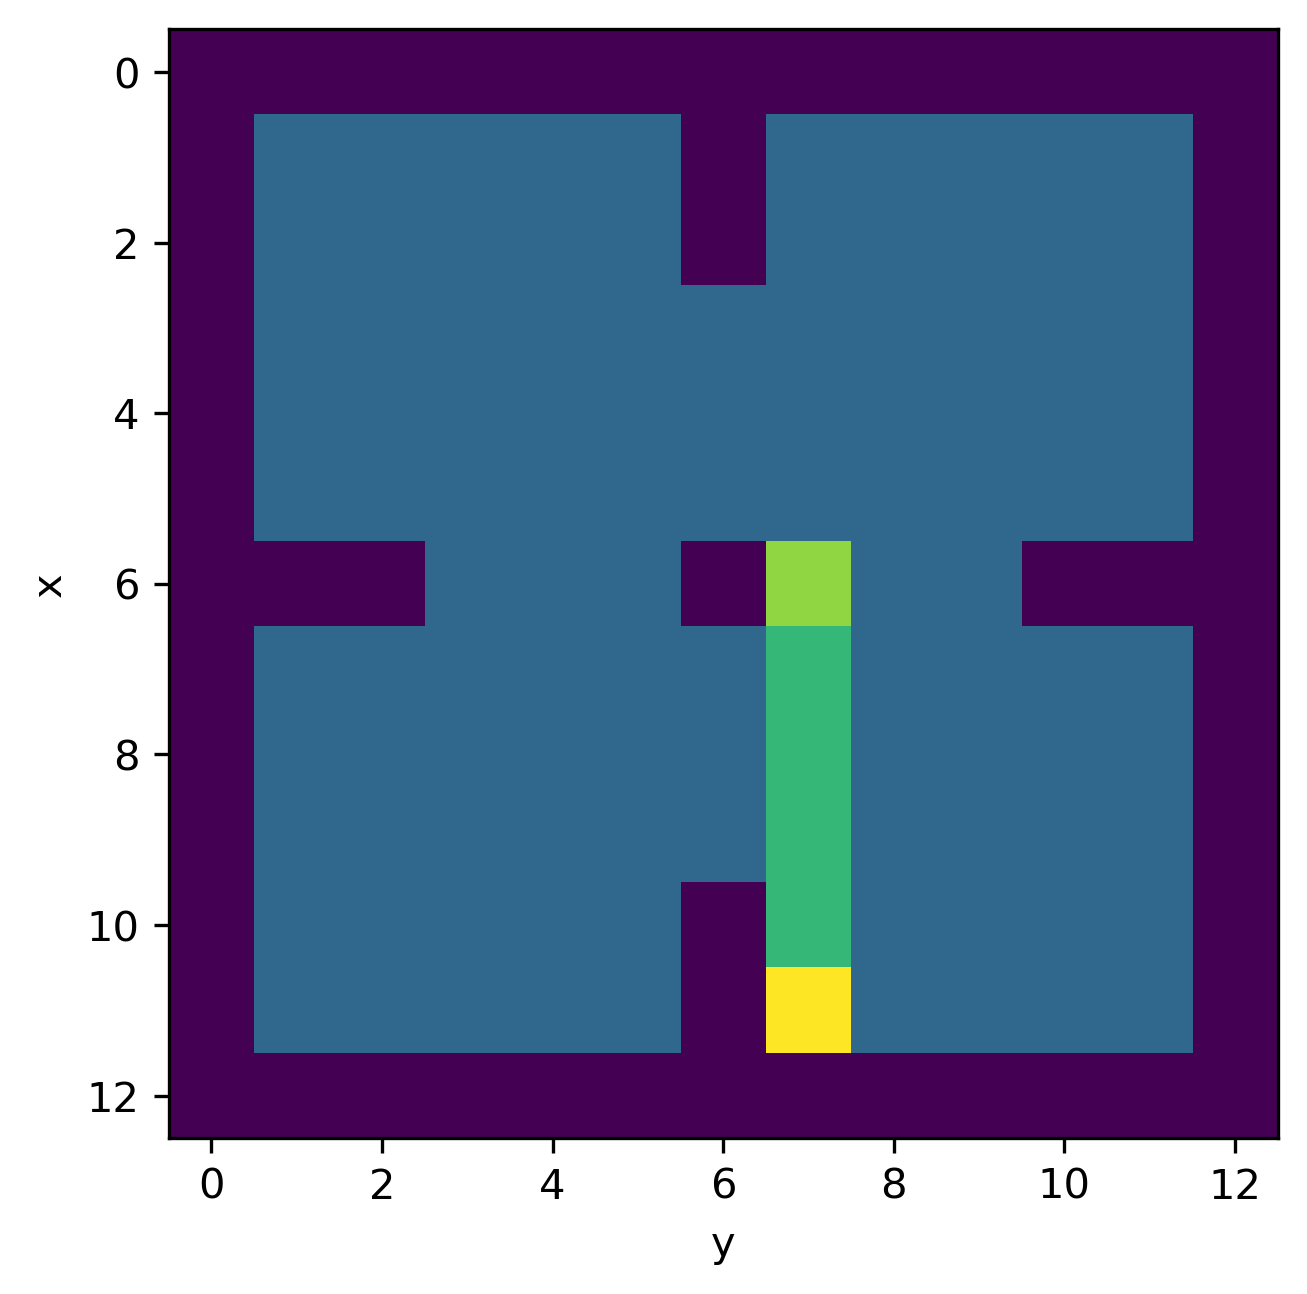
\includegraphics[height= 5cm, width=5cm]{p3-2-6}
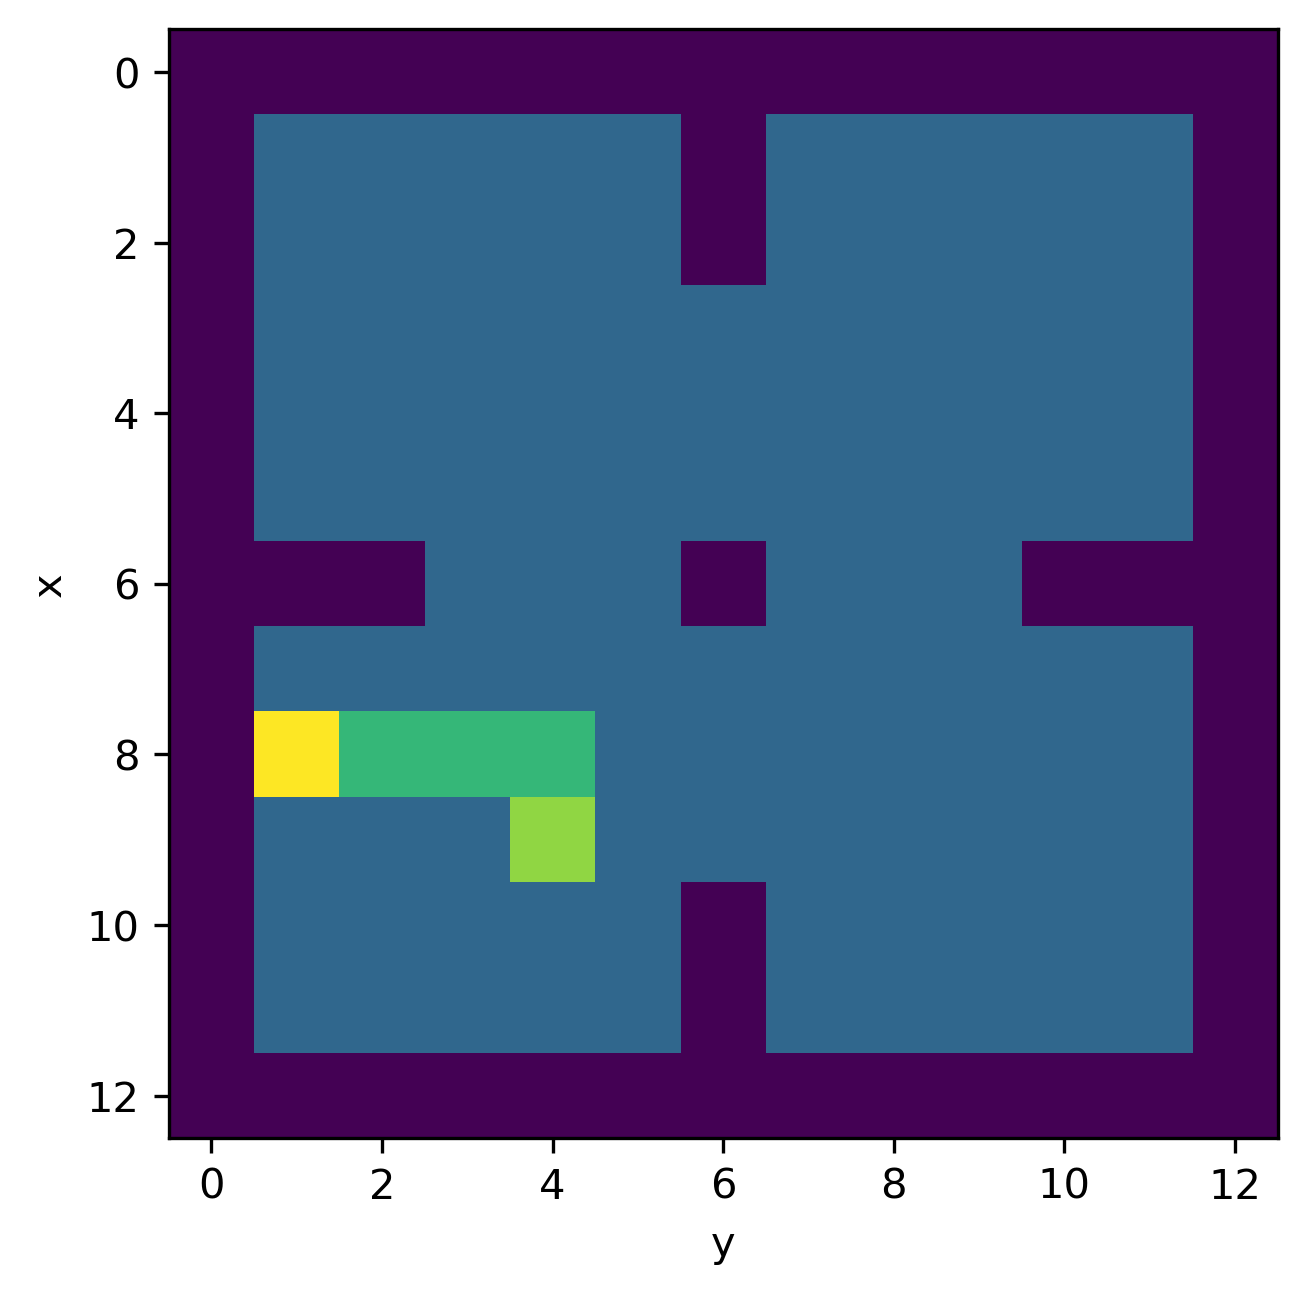
\includegraphics[height= 5cm, width=5cm]{p3-2-7}
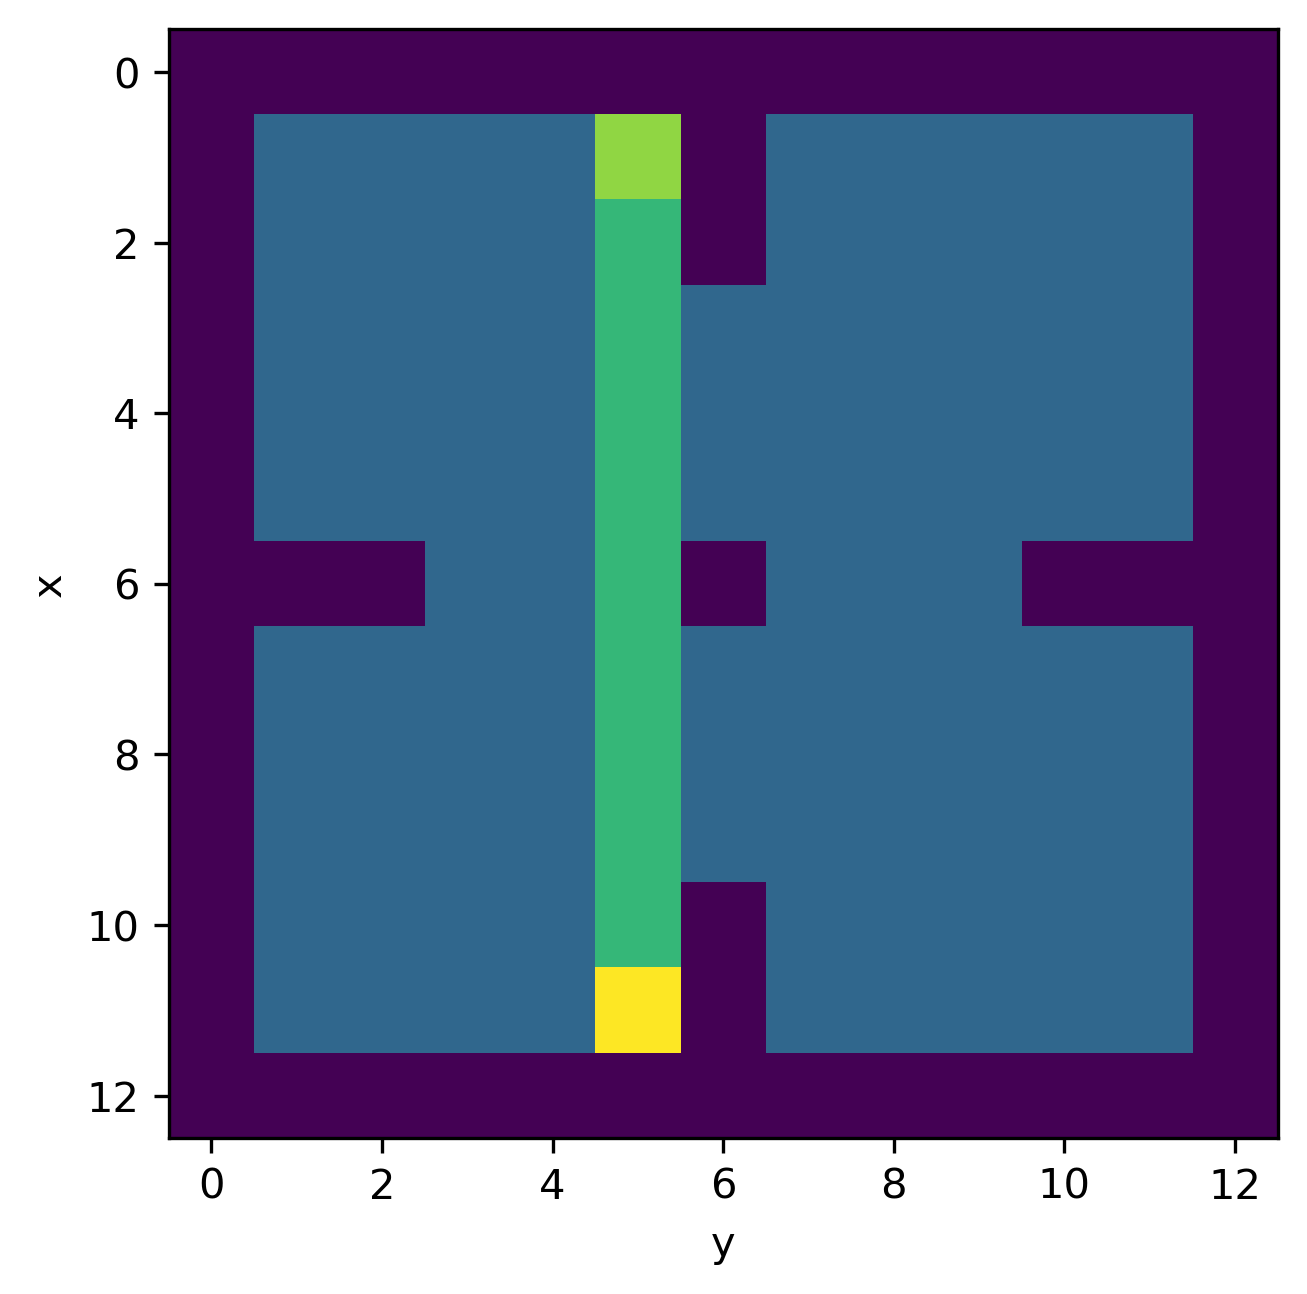
\includegraphics[height= 5cm, width=5cm]{p3-2-8}
\\
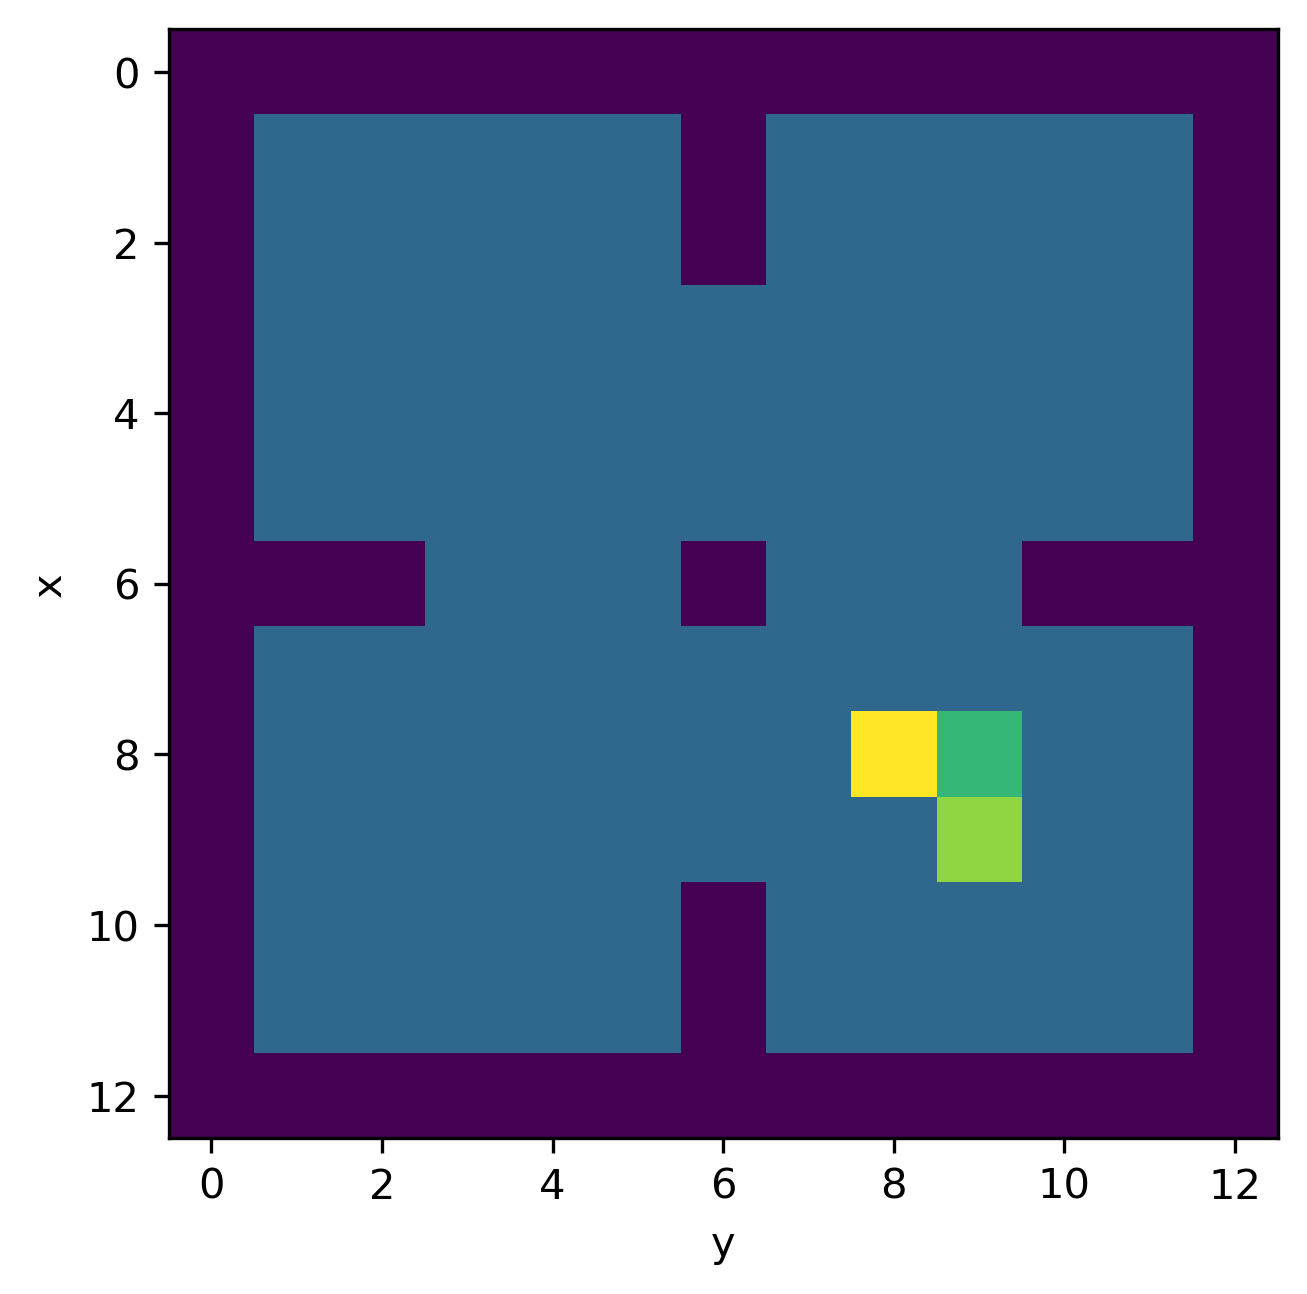
\includegraphics[height= 5cm, width=5cm]{p3-2-9}
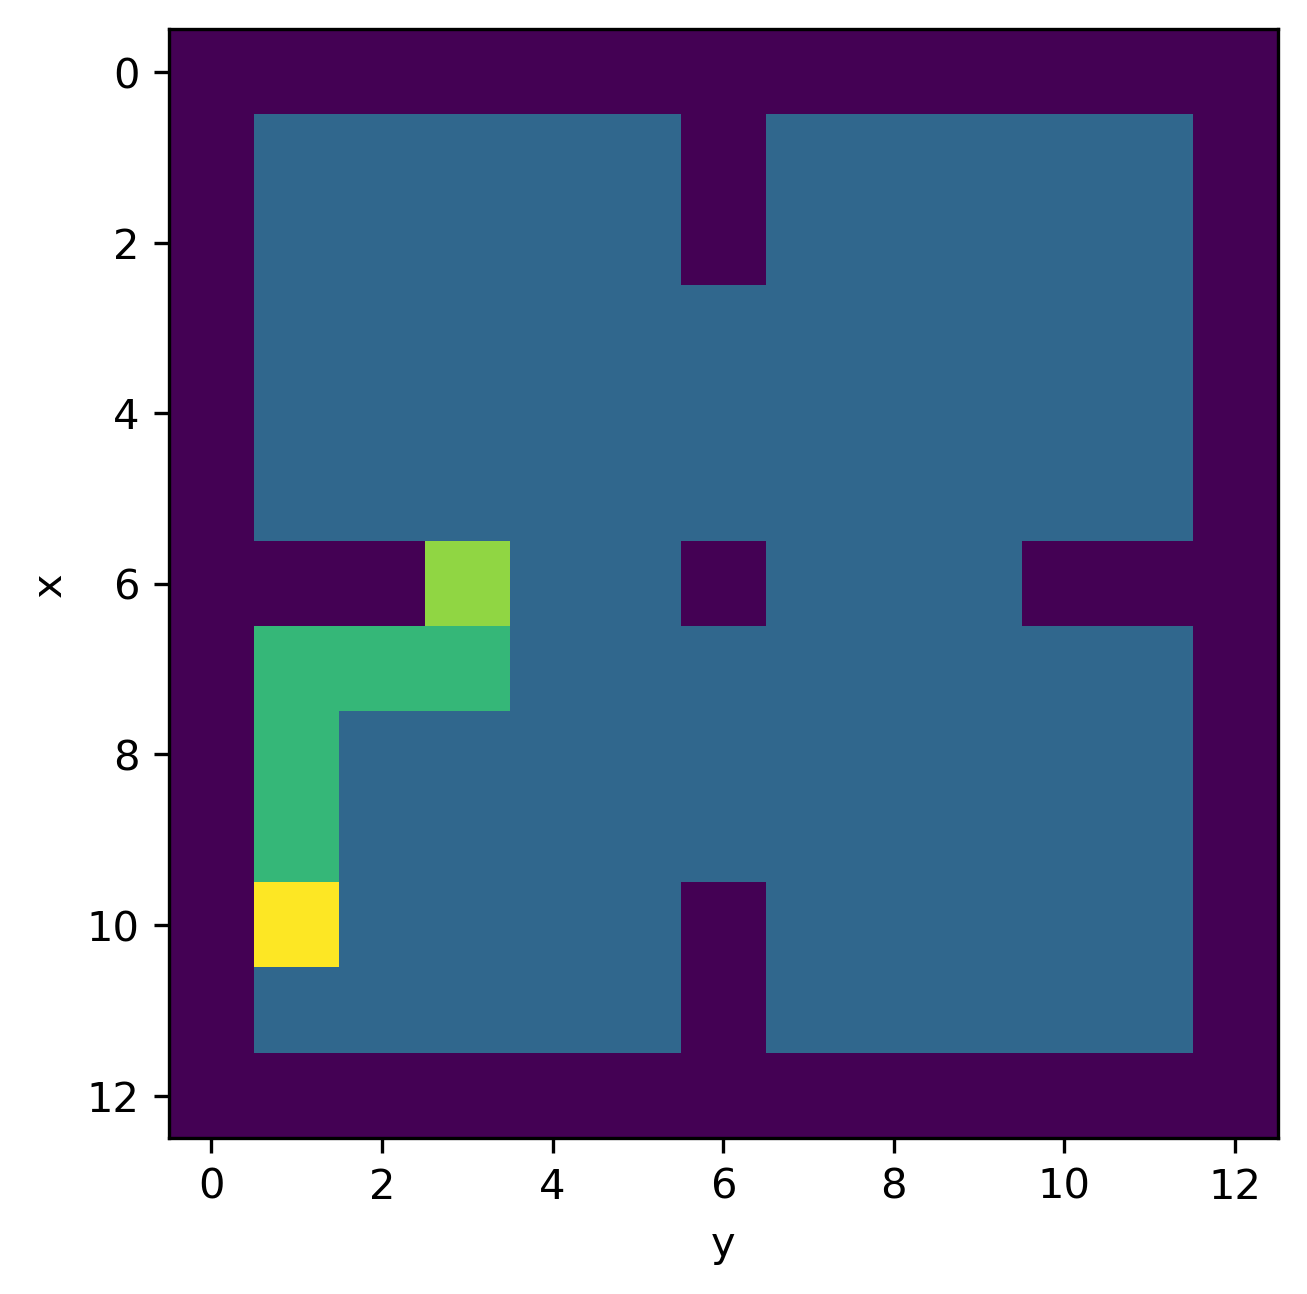
\includegraphics[height= 5cm, width=5cm]{p3-2-10}
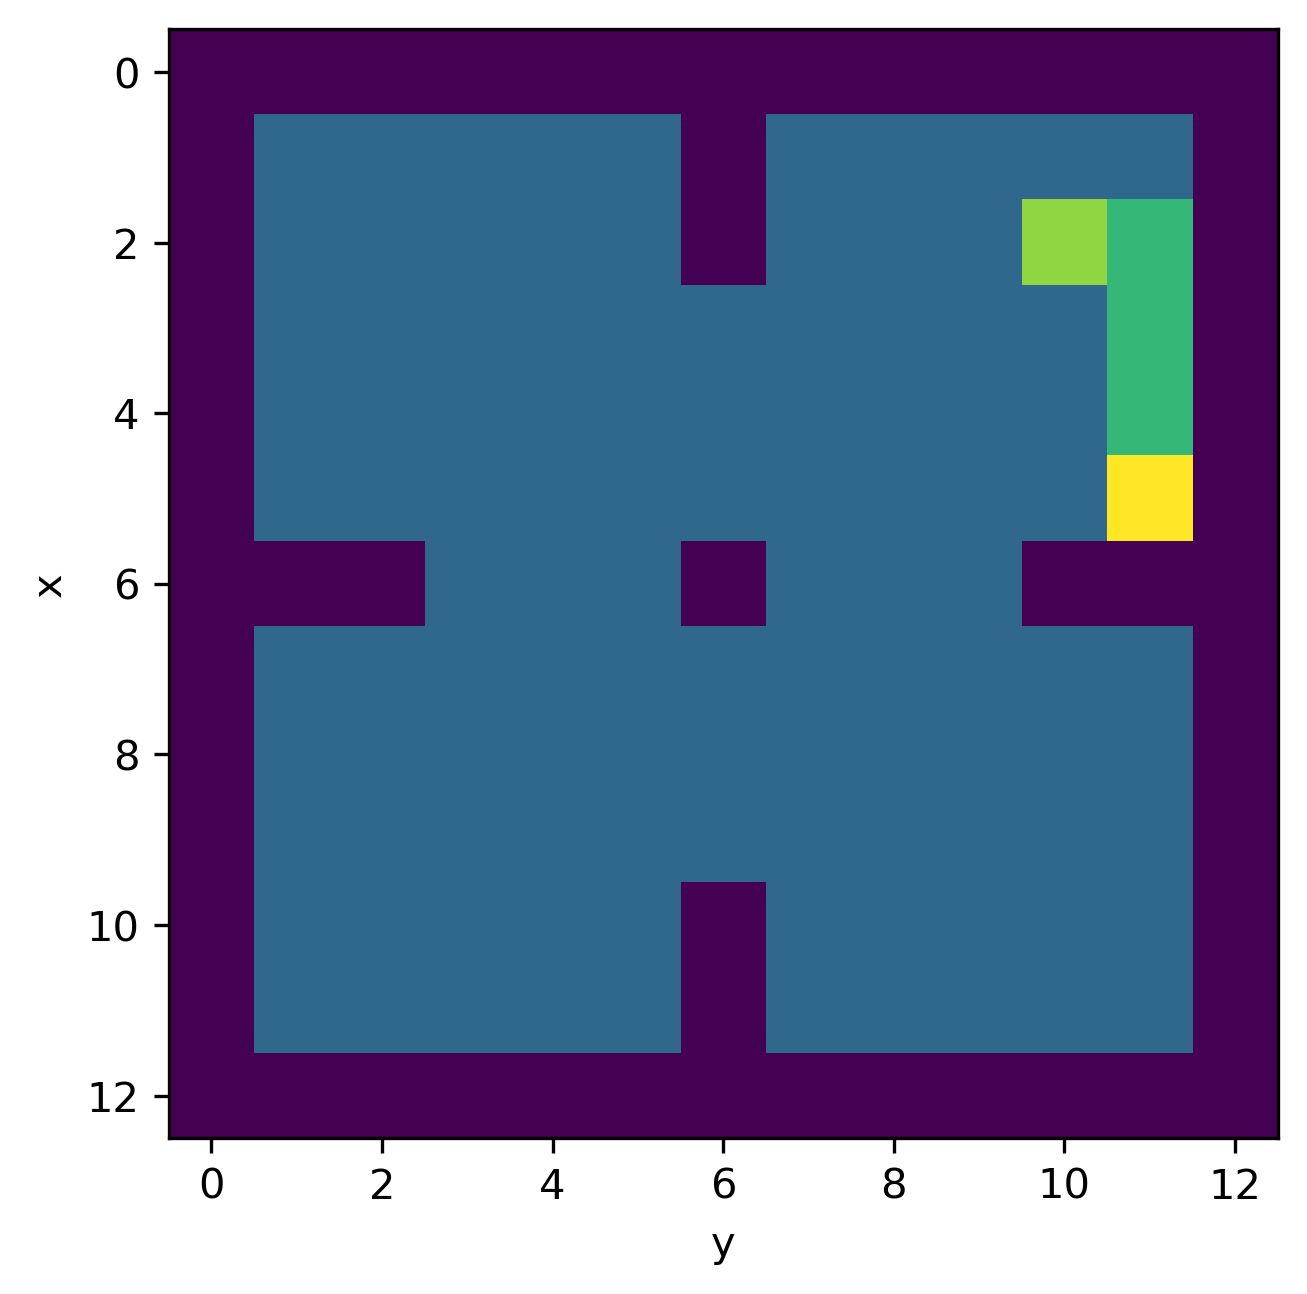
\includegraphics[height= 5cm, width=5cm]{p3-2-11}

\subsection*{3.3 Train Goal-Conditioned Policy via BC (10 pt)}

\begin{tcolorbox}[fit,height=22em, width=40em, blank, borderline={1pt}{1pt},nobeforeafter]
\begin{center}
%YOUR SOLUTION HERE%

\end{center}
\end{tcolorbox}




\subsection*{3.4 Expert Relabelling Trick (20 pt)}
\subsection*{3.4.1 From Expert Policy (10 pt)}

\begin{tcolorbox}[fit,height=22em, width=40em, blank, borderline={1pt}{1pt},nobeforeafter]
\begin{center}
%YOUR SOLUTION HERE%

\end{center}
\end{tcolorbox}


\subsection*{3.4.2 From Random Policy (10 pt)}

\begin{tcolorbox}[fit,height=50em, width=40em, blank, borderline={1pt}{1pt},nobeforeafter]
\begin{center}
%YOUR SOLUTION HERE%

\end{center}
\end{tcolorbox}


\subsection*{3.5 Conceptual Questions (4 pt)}

\begin{tcolorbox}[fit,height=22em, width=40em, blank, borderline={1pt}{1pt},nobeforeafter]
\begin{center}
%YOUR SOLUTION HERE%

\end{center}
\end{tcolorbox}

\section*{Extra (0 pt)}

\textbf{Feedback}: You can help the course staff improve the course by providing feedback. What was the most confusing part of this homework, and what would have made it less confusing?

\begin{tcolorbox}[fit,height=10em, width=40em, blank, borderline={1pt}{1pt},nobeforeafter]
            \begin{center}
            \end{center}
            \end{tcolorbox}\\

\noindent\textbf{Time Spent}: How many hours did you spend working on this assignment? Your answer will not affect your grade.

\begin{tcolorbox}[fit,height=8em, width=40em, blank, borderline={1pt}{1pt},nobeforeafter]
\begin{table}[H]
    \centering
    \begin{tabular}{r|c}
        Alone &  \hspace{3em}  %ANSWER HERE%  
        \\ \hline
        With teammates & \hspace{3em}  %ANSWER HERE%
        \\ \hline
        With other classmates & \hspace{3em}  %ANSWER HERE%
        \\ \hline
        At office hours & \hspace{3em}  %ANSWER HERE%
        \\ \hline
    \end{tabular}
        
\end{table}
\end{tcolorbox}

\end{document}
